\documentclass[11pt,british]{article}
\usepackage[T1]{fontenc}
\usepackage[latin9]{inputenc}
\usepackage{geometry}
\usepackage{pdfpages}
\usepackage{listings}
\lstset{language=VHDL}
\usepackage{babel}
\usepackage[justification=centering]{caption}
\usepackage{float}

%%%%%%%%%%%%%%%%%%%%%%%%%%%%%%
\usepackage{afterpage}
\newcommand\blankpage{%
    \null
    \thispagestyle{empty}%
    \addtocounter{page}{-1}%
    \newpage}
%%%%%%%%%%%%%%%%%%%%%%%%%%%%%%

\geometry{verbose,tmargin=1in,bmargin=1.5in,lmargin=2.5cm,rmargin=2.5cm,headheight=2.1cm,headsep=2.1cm,footskip=1in}
\exhyphenpenalty=10000\hyphenpenalty=10000
\makeatletter
\makeatother

%%%%%%%%%%%%%%%%%%%%%%%%%%%%%%%%%%%%%%%%%%%%%%%%%%%%%%%%%%%%
%% Title- & blank page
\begin{document}

%%Mandatory blank page
\newpage
\thispagestyle{empty}
\mbox{}

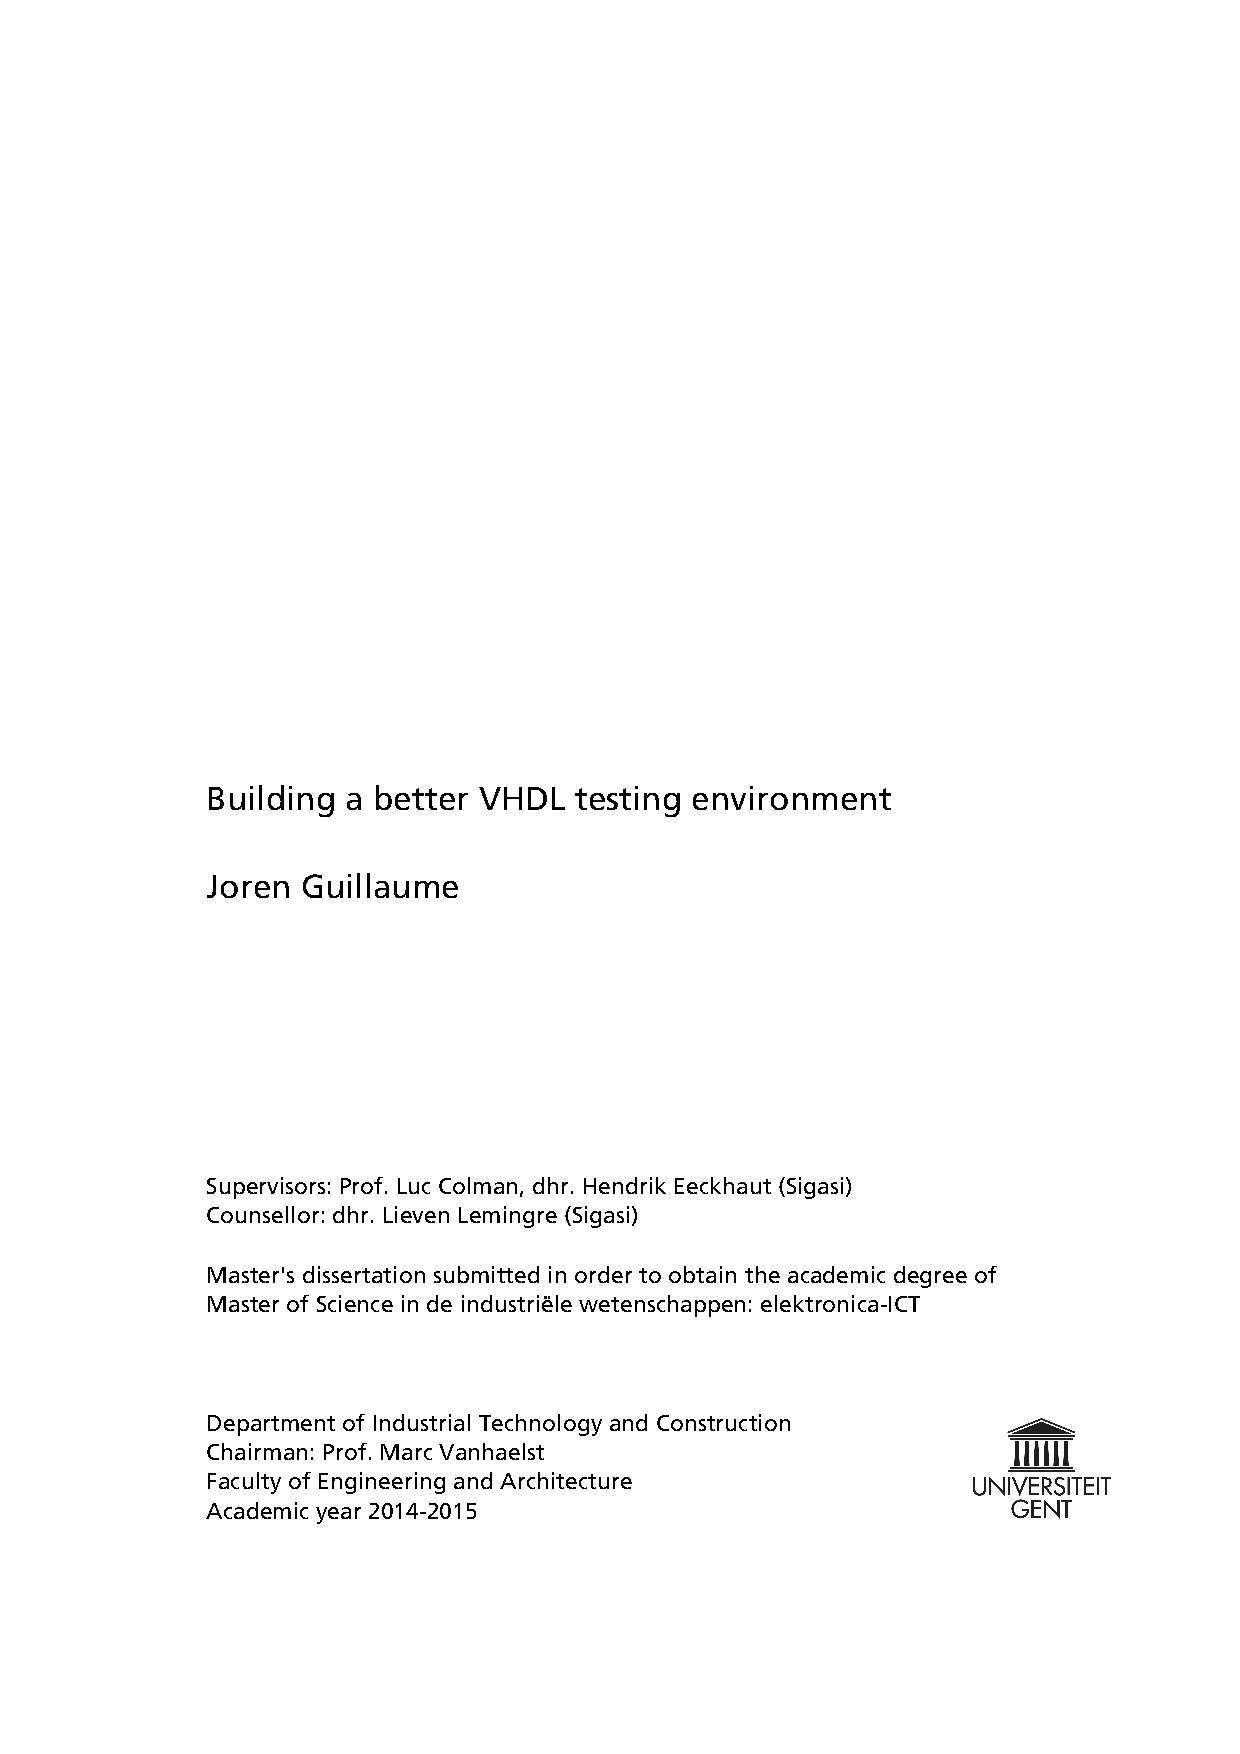
\includepdf[pages={1}]{title-generated.pdf}

%%%%%%%%%%%%%%%%%%%%%%%%%%%%%%%%%%%%%%%%%%%%%%%%%%%%%%%%%%%%
%% Preface

\newpage{}\part*{Preface}

\pagebreak{}

%%%%%%%%%%%%%%%%%%%%%%%%%%%%%%%%%%%%%%%%%%%%%%%%%%%%%%%%%%%%
%% Abstract

\newpage{}
\begin{abstract}
\pagebreak{}
\end{abstract}

%%%%%%%%%%%%%%%%%%%%%%%%%%%%%%%%%%%%%%%%%%%%%%%%%%%%%%%%%%%%
%%

\tableofcontents
\pagebreak

%%%%%%%%%%%%%%%%%%%%%%%%%%%%%%%%%%%%%%%%%%%%%%%%%%%%%%%%%%%%
%%

\listoffigures
\pagebreak

%%%%%%%%%%%%%%%%%%%%%%%%%%%%%%%%%%%%%%%%%%%%%%%%%%%%%%%%%%%%
%%

\listoftables
\pagebreak

%%%%%%%%%%%%%%%%%%%%%%%%%%%%%%%%%%%%%%%%%%%%%%%%%%%%%%%%%%%%

\part{Problem and background}


\section{Problem}

Developing VHDL, like any code, is prone to error creation, either
by user or by wrong product specifications. To ensure errors are weeded
out before the more expensive production begins, the code is subjected
to rigorous testing. For full product testing by conventional means,
large and impractical tests are needed.
\\
\\
Because testing is such a time consuming process, finding errors often
results in severe delays due to the need to both correct the error
and test for others. Therefore it is in the best interests of both
testing engineers and software engineers to find and correct errors
with minimal delay and maximal effort. This process should affect
the least amount of code possible as to minimize time spent retesting
and recoding.
\\
\\
In this thesis, a number of mechanics are used to optimize both testing
and coding. Based loosely off of Test Driven Development (TDD), tests
are written to both function and be tested independently to maximize
test coverage with minimal effort. To this end, a library with often
used functions and other useful code is made available. Alongside
of it is a tool, written in Python, to process tests made with this
library independently and represent the results in a quick and easy
to read format.
\\
\\


\newpage{}


\section{Introduction}


\subsection{Digital Electronics}

There are two kinds of electronic appliances and circuits, digital
and analogue. Digital electronics differ from analogue electronics
in that they use a discrete set of voltage levels to transmit signals.
The most common number of items in the set is 2, a level for one (commonly
named ``high'') and a level for zero (commonly named ``ground''
or ``low''). The advantage of using a discrete number of levels
rather than a continuous signal as is used in analogue electronics
is that noise generated by the environment, thermal noise and other
interfering factors, will have but a minor influence on the signal.\\


To process these discrete signals, electronics are made up of transistors
that nowadays are formed in with the \emph{Complementary Metal Oxide
Semiconductor }(CMOS) technology. This technology uses both an \emph{NPN}
and a \emph{PNP} transistor that work in a push-pull configuration.
The p's and n's in NPN and PNP simply stand for \emph{Positive} and
\emph{Negative}, they are made of positive and negative doped lumps
of semiconductor (usually Silicon-Dioxide or SO$_{2}$). A transistor
is basically a blockade on a track and depending on the force applied
to its Gate, it opens or closes the track.\\


In reality, the force takes form of a current and an NPN transistor
opens its gate when a positive current is applied. A PNP transistor,
however, always leaves its gate open until a current is applied. This
means that if we send the same signal to an NPN and a PNP transistor,
with one of the signals inverted, we can open and close two parts
of the entire circuit at the same time. This is useful to both direct
a certain signal to ground and at the same time close its connection
with the \emph{source} (the power source). Hence also the name \emph{Complementary}
MOS, the NPN and PNP complement each other.

A certain combination of transistors is used to make \emph{logic gates}.
These logic gates make it so that only a certain combination of ones
and zeroes at the inputs result in certain ones or zeroes at the outputs.
For instance, one of the most common logic gates is a \emph{nand }gate
(a \emph{not and }gate). This gate has a number of inputs ranging
from 2 to theoretically infinity (but practically 3 or 4) and only
outputs a low\emph{ }signal if all of the inputs are \emph{high} (digital
one), otherwise its output is \emph{at ground} or \emph{low} (digital
zero). The other most common logic gate is the \emph{nor }gate (a
\emph{not or }gate). This gate outputs a low signal if any of its
inputs are high, otherwise it outputs a low.

A common mistake is to think that low or ground mean \emph{zero voltage.}
This is only partially true, the high signals are measured with ground
as their reference. So a high signal of 1.8 Volts would be 1.8 Volts
higher than ground, and could be considered to be at 1.8 Volts if
ground is the theoretical zero.

A certain combination of these logic gates are used to build higher-level
blocks such as flip-flops, which are used to make registers and so
on up to the entire chip design.


\subsection{Hardware Description Languages}

A \emph{Hardware Description Language} (HDL) can be used to describe
any one of these levels, right down to the logic gate level, however
this last one might not be a good idea considering most synthesis
tools can produce superior logic gate-level layouts\cite{key-1}.
The level that uses certain blocks of logic gates to describe more
complex behaviour is called the \emph{Register Transfer Level} or
RTL. Some blocks are standard implementations that have been widely
used and nearly fully optimized, such as memories, flip-flops and
clocks. An RTL flip-flop implementation is shown here: 

\begin{lstlisting}[tabsize=4, frame=single]
library IEEE;
use IEEE.std_logic_1164.all;
entity DFF is
	Port(D 	 : in std_logic;
		 CLK : in std_logic;
		 Q 	 : out std_logic;
end DFF;

architecture Behavioural of DFF is
begin
	process (CLK)
	begin
		if rising_edge(CLK) then
			Q <= D;
		end if;
	end process;
end Behavioural;
\end{lstlisting}

The IEEE library provides a number of extensions on the original VHDL
code that allow a more realistic simulation and description of hardware
behaviour. An entity defines the inputs and outputs of a certain building
block, in this case the D Flip-flop or DFF. The D stands for Delay,
and it simple puts on its output Q that which was on the input one
clock cycle earlier. The architecture, in this case Behavioural, takes
the description of an entity and assigns a real implementation to
it. All processes are executed in parallel, this does not mean that
all are triggered at the same time, nor do they take as long to finish,
but it means that any process can be executed alongside any other
process. In this case there is only one (nameless) process that describes
the entire behaviour of the flip-flop. It waits for the rising edge
of the clock, which is a transition from zero to one, and then it
schedules the value of D to be put on Q until the next rising edge
appears.

This is a basic example of an entity, an architecture and a process.
This flip-flop could be used in certain numbers to build a \emph{register},
a collection of ones and zeroes (henceforth named \emph{bits}) that
is used to (temporarily) store these values. The register could then
be used alongside combinational logic to build an even bigger entity.
The idea here is that small building blocks can be combined to produce
vast and complex circuits that are nearly impossible to describe in
one go. Adding all these layers together also creates a lot of room
for error, and having a multi-level design makes it somewhat difficult
to pinpoint the exact level and location of any errors. Therefore
it is paramount that all code on all levels is tested thoroughly,
this is done by use of \emph{testbenches}.\cite{key-2}

Testbenches are made up of code that takes a certain building block,
the \emph{Unit Under Test} (UUT) or \emph{Device Under Test} (DUT).
The testbench then performs a certain sequence of inputs and monitors
the outputs. If the device performs normally, the received output
sequence should match a certain \emph{golden reference}, the expected
output sequence. In these testbenches it is also interesting to see
how well a device performs if its inputs behave outside the normal
mode of operation. When all of these tests have finished and the output
performs as expected, the device is ready to be put into production
or further down the developmental process.

It is easy to see that if a device is not tested properly and faults
propagate it can be very expensive to correct, especially at the stage
of production, where a single photomask, used to ``print'' part
of the layout, can easily cost \$100,000\cite{key-3}. Therefore a
large portion of time is spent writing and executing tests\cite{key-4}.
Practices to improve both the speed and quality of testing and coding
exist in a large number, but the focus chosen in this thesis is \emph{Test
Driven Development} (TDD). This practice has proven to increase test
coverage\cite{key-5}, decrease defect density\cite{key-8} as well
as improve code quality\cite{key-9,key-8}.


\section{Mission and objectives}

The goal of this thesis is to ease development and testing of VHDL
code, with a focus on testing and test reporting. Practically this
means the development of several tools which can be independently
used and each have their own merit.
\begin{itemize}
\item A testbench parser that ensures independent testing and proper test
report generation.
\item A library with many widely-used functions as to speed up programming,
as well as functions to make reporting possible.
\item A test report that can easily be read but still holds a significant
amount of detail on errors and successes.\end{itemize}


\pagebreak{}
\begin{thebibliography}{1}
\bibitem{key-1}http://www.asic-world.com/vhdl/intro1.html

\bibitem{key-2}Writing Testbenches: Functional Verification of HDL
Models

\bibitem{key-3}Mask Cost and Profitability in Photomask Manufacturing:
An Empirical Analysis

\bibitem{key-4}Citation needed !!

\bibitem{key-5}A comparative case study on the impact of test-driven
development on program design and test coverage

\bibitem{key-8}A Longitudinal Study of the Use of a Test-Driven Development
Practice in Industry

\bibitem{key-9}Evaluating the Efficacy of Test-Driven Development\end{thebibliography}

%%%%%%%%%%%%%%%%%%%%%%%%%%%%%%%%%%%%%%%%%%%%%%%%%%%%%%%%%%%%
%% 

\newpage{}
\part{Appendix}

%%%%%%%%%%%%%%%%%%%%%%%%%%%%%%%%%%%%%%%%%%%%%%%%%%%%%%%%%%%%
%% Mandatory blank page

\afterpage{\blankpage}


\end{document}
